\documentclass[a4paper,10pt]{scrartcl}
\usepackage[ngerman]{babel}
\usepackage[T1]{fontenc}
\usepackage[utf8]{inputenc}
\usepackage{graphicx} 

\title{Software Engineering 3}
\author{Benjamin Altmiks}
\date{8. Oktober 2018 - \today}

\begin{document}
\tableofcontents
\maketitle

\section{Einleitung}
\subsection{Rückblick}
        \textbf{Zeit:}      Bei Zeit wird Start und Enddatum/Stunde verwendet. Es ist nicht relevant wie viele Personen an dem Projkt beteiligt waren.
\newline\textbf{Kosten:}    Äquivalent zur Zeit, da die Areitszeit bezahlt werden muss. 
                                Hier ist es relevant wie viele Personen an diese Projekt gearbeitet haben da ealle bezahlt werden müssen.
\newline\textbf{Qualität}:   Unterscheidung zwischen Produktqualität und Prozessqualität.
\begin{itemize}
    \item Produktqualität: Der ganze Prozess, das beeinhaltet Brauchbarkeit und Wartbarkeit 
    \item Prozessqualität: Das Endprodukt, das Ergebniss, das heißt die Software selber
\end{itemize}
\section{Architektur}
\subsection{Allgemein}
\begin{quote}   "Architektur ist schwer greifbar" \newline -Vogel   \end{quote}
Architktur ist ein sich selbst durch die Evolution entwicklender Prozess. Sie ist ein universeller Bestandteil/Grundriss von Software
\begin{quote}    "... werden Entwickler, wenn auch oft unbemerkt, in ihrer täglichen Arbeit mit Architektur konfrontiert, weil diese impliziet immer ein Aspekt von
Software ist und sich nicht eliminieren, allenfalls ignorieren lässt." \newline -Vogel    \end{quote}
\textbf{Softwarearchitektur ist eine strukturierte oder hierarchische Anordnung der Systemkomponenten sowie Beschreibung ihrer Beziehungen. Diese nennt man häufig Architekturmuster}
\newpage
\subsection{Architekturmuster}
Architekturmuster versuchen eine grundlegede Organisation und Interaktion zwischen Komponenten einer Anwendung her zu stellen. Man unterscheidet allgemein Strukturierende Architekturmuster, Muster für Interaktive Systeme und Muster für verteilte Sytsteme

\subsubsection{Strukturierende Architekturmuster}
\textbf{Pipes und Filter}
\begin{itemize}
    \item Beschreibt die Struktur für Systeme, die Datenströme verarbeiten.
    \item Filter = Verarbeitungsschritt mit Dateneingabe und Datenausgabe
    \item Pipes = Verbindung zwischen einzelner Komponenten \newline
    $\Rightarrow$ Verschiedene, unabhängige Komponenten für flexible, unterschiedliche Aufgaben
\end{itemize}
\textbf{Schichten}
\begin{itemize}
    \item Aufteilung auf Schichten für große/komplexe Systeme 
    \item Ziel ist eine Abhängigkeitslösung der Komponenten zu erreichen\newline
    $\Rightarrow$ Austauschbarkeit und Integration neuer Systeme einfacher möglich
    \item Ein Besipiel ist das OSI-Schichtenmodell bei Netzwerkprotokollen
\end{itemize}
\subsubsection{Architekturmuster für interaktive Systeme}
\textbf{Model-View-Controller}\newline
Einteilung in drei Komponenten:
\begin{enumerate}
    \item Datenmodell (model): Enthält die Daten die dargestellt werden. Ist unabhängig von anderens
    \item Präsentation (view): Darstellung der Daten des Modells mit Benutzerinteraktion
    \item Programmsteuerung (controller): Benutzerinteraktionen verwaltet Präsentation und Datenmodell
\end{enumerate}
$\Rightarrow$ Reduzierung von Abhängigkeiten, Benutzerschnittstellenorientiert  \newline
\begin{figure}[h]
	\centering
	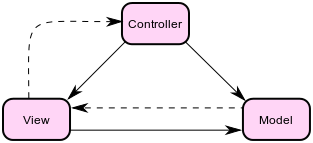
\includegraphics[width = 4.5cm]{ModelViewControllerDiagram2}
\end{figure}
\newpage
\subsubsection{Architekturmuster für verteilte Systeme}
\textbf{Vermittler-Prinzip}

\begin{itemize}
    \item Verteiltes System mit (unabhängigen) Komponenten, die zusammenarbeiten 
    \item Vermittler steuert Objekte, Objekte nicht untereinander\newline
    $\Rightarrow$ Einfache Kombination von Diensten und Objekten in einem System
\end{itemize}
\textbf{Client-Server}
\begin{itemize}
    \item Verteilte Benutzer mit zentraler Anwendung 
    \item Verschiedene Funktionalitäten durch Verteilung auf Netzwerkkomponenten\newline
    $\Rightarrow$ Beispiele sind das WWW oder E-Mail 
\end{itemize}
\subsubsection{Zusammenfassung}
\begin{itemize}
    \item Architektur bringt keinen direkten Mehrwert für die Software mit sich
    \item Funktionale Zusätzliche Fähigkeiten und Flexibilität der Software besser\newline
    $\Rightarrow$ Zukunftssichere Software (Kostengünstiger, Zuverlässiger)
    \item Gute Architektur ist eine notwendige, aber keine hinreichende Voraussetzung für gute Qualität
\end{itemize}
\subsection{Micro- und Marko Architektur}
Allgemein werden beide benötigt um die Effizienz des Entwicklungsprozesses zu verbessern.
\subsubsection{Microarchitecture TODO}
Micro Architektur betrachtet die Software Entwicklung „von Unten”, legt also den Fokus auf auf
kleine Einflüsse.
\begin{itemize}
    \item \textbf{FUTUR} Eine Future stellt der Rückgabewert einer Berechnung dar, der zur Zeit noch nicht verfügbar ist.
    \item \textbf{CALLBACK}
    \item \textbf{LISTENABLEFUTURE}  Kombination aus Future und Callbacks
    \item \textbf{PROMISES}
\end{itemize}

\subsubsection{Event}
Ein Ereignis (englisch Event) dient in der Softwaretechnik – bei Entwicklung nach dem ereignisorientieren Programmierparadigma – zur Steuerung des Programmflusses. Das Programm wird nicht linear durchlaufen, sondern es werden spezielle Ereignisbehandlungsroutinen (engl. listener, observer, event handler) immer dann ausgeführt, wenn ein bestimmtes Ereignis auftritt. Ereignisorientierte Programmierung gehört zu den parallelen Programmiertechniken, hat also deren Vor- und Nachteile.
\begin{itemize}
    \item + Sehr einfach neue Systeme umzusetzten 
    \item + Jedes abhängige System kann seine Sicht auf die Daten vorhalten. Vermeidung von „Resource contention”
    \item - Es ist nicht einfach, festzustellen, welche Systeme voneinander abhängen
    \item - Konsistenz: Die Datenmodelle sind nur noch „eventually consistent”
\end{itemize}
$\Rightarrow$ Events werden generiert wenn eine Veränderung am Datenmodell vorgenommen wurde. 
\subsection{Architektur Dokumentieren}
\subsubsection{Wie viel Architektur Dokumentation ist sinnvoll?}
Man muss berücksichtigen:
\begin{itemize}
    \item Nutzen des Dokuments für Entwickler, neue Mitglieder des Teams, etc.
    \item Den Aufwand, das Dokument zu pflegen
\end{itemize}
$\Rightarrow$ Wägen Sie für jedes Projekt ab, welche Dokumentation sinnvoll ist.
\subsubsection{Feste Gliederung}
\textbf{Vorteile}: Einheitliche Gliederung für alle Autoren mit einfacher Vollständigkeitssicherung. Neue Mitglieder und Reviews einfacher. \\
\textbf{Nachteile}: Form über Inhalt, Vollständigkeitsmengel\\
\subsubsection{arc42}
\begin{itemize}
    \item Aufgabenstellung: Architektur Dokumentation über Schach-Engine
    $\Rightarrow$ Feauters sind Schachregeln, Taktiken, User vs AI oder AI vs AI, Integration
    \item Qualitätsziele
    $\Rightarrow$ Analysierbarkeit, Änderbarkeit, Interoperabilität, Attraktivität
    \item Stakeholder
    $\Rightarrow$
\end{itemize}

\subsection{Testen und Verifizieren}
\subsubsection{Software-Qualitätssicherung}
Fehler können immer auftreten. Dazu werden Softwar-Prüfungen durchgeführt, um die Qualität noch weiter zu verbessern. Man unterscheidet zwischen:
\begin{itemize}
    \item Dynamischen Tests\\
    $\Rightarrow$ Manuelles Testen des Menschen\\ 
    $\Rightarrow$ Automatisches testen von einem Rechner
    \item Statische Tests\\
    $\Rightarrow$ Manuelle Verfahren sind dabei Verifikationen und Code Reviews\\
    $\Rightarrow$ Auomatische Verfahren können Coding Conventions, statische Analysen oder automatische Verifikationen sein
\end{itemize}
$\Rightarrow$ Das Ziel ist möglichst viele Fehler zu finden und diese zu reparieren.
\subsubsection{Fehler - Definition und Abgrenzung}
\begin{table}[h]
    \begin{tabular}{|l|l|l|} \hline
Begriff & Erklärung & Erkennbarkeit/Lösung \\\hline
Fehlerbedienung & Falsche Bedienung durch Nutzer & Handbuch/Fehlermeldung\\\hline
Defekt & Fehlerhafte Stelle &               \\\hline
    \end{tabular}
\end{table}
\subsubsection{Vom Fehler zum Defekt}
Das Allgemeine Vorgehen zum Lösen eines Fehlers
\begin{enumerate}
    \item Breakpoint setzten und Fehlverhalten immer weiter eingrenzen
    $\Rightarrow$ Oft gibt es viele Infizierte Stellen
    \item Je größer die Software, desto schwerer ist abzuschätzen wo der Fehler ist.
    \item 
    \item 
\end{enumerate}
\subsubsection{Korellation vs Kausalität}
Korellation: Zwei oder mehrere Merkmale müssen keine Beziehung zueinander haben. Sie beeinflussen sich gegenseitg nicht, können aber eine Zufällige Beziehung zueinander haben.
Kausalität: Eine Ursache-Wirkung Beziehung, betrifft also die Abfolge aufeinander bezogener Ereignisse und Zustände.
\subsubsection{Defekte finden}
\begin{enumerate}
    \item \textbf{Asserts}: 
    Teil eines Programms welches eine Erwartung ausdrückt. Speicherstellen werden gegen erwartete Werte getestet. (In Java mit 'assert + boolschen Ausdruck' oder mit Assert.statischeMethoden(boolean))\\
    $\Rightarrow$ Aber keine zu (zeit)aufwendigen Asserts, da bei einer Aktivierung der Asserts ein veränderter Zeitlicher Ablauf stattfinden kann.
    \item \textbf{Unit-Tests}: 
    \item \textbf{Integrations-Tests}:
    \item \textbf{Logs/Tracers}:
\end{enumerate}
\subsection{Java Modelling Language (JML)}
Mithilfe von JML können Vor- und Nachbedingungen 

\subsubsection{Funktionsorientierte Tests}

\end{document}
